\documentclass[../main.tex]{subfiles}
\begin{document}
\chapter{Tipe Data, Variabel, dan I/O}

\section*{Tujuan Praktikum}
Setelah menyelesaikan praktikum ini, mahasiswa diharapkan mampu:
\begin{itemize}
  \item Memahami berbagai tipe data dasar (integer, real, char, boolean) di Pascal, C, dan C++
  \item Mendeklarasikan dan menginisialisasi variabel dengan tipe data yang tepat
  \item Memahami batasan dan rentang nilai setiap tipe data
  \item Melakukan operasi input dan output data menggunakan fungsi/prosedur yang sesuai
  \item Memformat output data dengan presisi dan lebar field yang diinginkan
  \item Membuat program interaktif sederhana dengan input dari pengguna
  \item Menjelaskan model data umum (LP64 vs LLP64) dan dampaknya terhadap ukuran tipe
  \item Menggunakan tipe bilangan tetap-lebar (\texttt{int32\_t}, \texttt{uint64\_t}) saat diperlukan \parencite{c-std-integer-types}
  \item Memilih format string yang benar pada C (\texttt{printf}/\texttt{scanf}) \parencite{c-printf,c-scanf}
\end{itemize}

\section{Tipe Data Dasar}
Tipe data adalah blueprint yang menentukan jenis nilai apa saja yang dapat disimpan dalam variabel dan operasi apa yang valid untuk dilakukan. Bahasa Pascal menyediakan tipe-tipe seperti \texttt{integer}, \texttt{real}, \texttt{char}, dan \texttt{boolean}. Di sisi lain, C dan C++ menawarkan \texttt{int}, \texttt{double}, \texttt{char}, serta \texttt{bool}. Perlu diingat bahwa ukuran sebenarnya dari tipe-tipe ini bisa berbeda tergantung platform yang digunakan, sehingga pemahaman tentang model data yang diadopsi menjadi sangat krusial \parencite{pascal-tutorial-wikibooks,iso-c-draft-n1570,cpp-arithmetic-types,cpp-fundamental-types}.

Memilih tipe data yang sesuai bukan hanya membuat kode lebih mudah dipahami, tetapi juga membantu compiler dalam melakukan optimasi. Dalam C/C++, kita bisa menggunakan modifier seperti \texttt{signed/unsigned} atau \texttt{short/long} untuk menyesuaikan rentang nilai. Sementara di Pascal, pendefinisian rentang indeks secara eksplisit membantu memperjelas batasan yang diharapkan dari sebuah variabel. Untuk informasi lengkap mengenai ukuran dan standar, dokumentasi resmi dari masing-masing bahasa menjadi rujukan terbaik \parencite{free-pascal-docs,iso-c-draft-n1570,cpp-reference}.

Memahami bagaimana data direpresentasikan di memori dan bagaimana konversi tipe terjadi secara implisit sangat penting untuk menghindari loss of precision. Sebagai contoh, dalam bahasa C, integral promotion dapat mengubah hasil dari sebuah ekspresi ketika tipe data yang berbeda dikombinasikan. Aturan praktis yang konservatif: lakukan type casting secara eksplisit hanya ketika memang diperlukan \parencite{gnu-c-manual,cpp-reference}.

\subsection{Model Data Umum (LP64 vs LLP64)}
Pada sistem 64-bit, ukuran dari tipe data integer bergantung pada model data yang diterapkan oleh sistem operasi. Model \textbf{LP64} yang digunakan di Linux dan macOS membuat tipe \texttt{long} berukuran 64-bit. Sedangkan model \textbf{LLP64} yang diadopsi Windows mempertahankan \texttt{long} pada ukuran 32-bit, namun menyediakan \texttt{long long} dengan ukuran 64-bit. Untuk memastikan ukuran tipe data di platform Anda, gunakan operator \texttt{sizeof}. Saat bekerja dengan binary interface atau file format, pertimbangkan untuk menggunakan tipe fixed-width agar lebih portable \parencite{wikipedia-data-models,cpp-fundamental-types}.

\begin{table}[H]
  \centering
  \caption{Perbandingan ukuran tipe integer (umum, ringkas)}
  \small
  \begin{tabular}{@{}llll@{}}
    \toprule
    Tipe & ILP32 (32-bit) & LP64 (Unix 64-bit) & LLP64 (Windows 64-bit) \\
    \midrule
    \texttt{int}       & 32 & 32 & 32 \\
    \texttt{long}      & 32 & 64 & 32 \\
    \texttt{long long} & 64 & 64 & 64 \\
    \bottomrule
  \end{tabular}
  \\\parencite{wikipedia-data-models}
\end{table}

\subsection{Tipe Bilangan Tetap-Lebar di C/C++}
Untuk mengatasi variasi ukuran tipe data antar platform, header \texttt{<stdint.h>} di C (atau \texttt{<cstdint>} di C++) menyediakan tipe data dengan ukuran yang terjamin, seperti \texttt{int32\_t} dan \texttt{uint64\_t}. Header ini juga mendefinisikan konstanta batas seperti \texttt{INT32\_MAX} dan sejenisnya. Penggunaan tipe-tipe ini sangat direkomendasikan ketika Anda perlu memastikan portabilitas, terutama dalam konteks format data atau protokol komunikasi \parencite{c-std-integer-types,cpp-numeric-limits}.

Contoh di bawah ini memperlihatkan bagaimana tipe fixed-width digunakan untuk menjamin konsistensi ukuran variabel di berbagai platform:

\begin{lstlisting}[language=C, caption={Contoh penggunaan <stdint.h> di C}]
#include <stdint.h>
#include <stdio.h>

int main(void) {
  int32_t a = 12345;    // selalu 32-bit signed
  uint64_t b = 1000000; // selalu 64-bit unsigned
  printf("%" PRId32 " %" PRIu64 "\n", a, b); // butuh <inttypes.h>
  return 0;
}
\end{lstlisting}

Dalam C++, tipe fixed-width dapat dikombinasikan dengan library \texttt{<limits>} untuk mengetahui batasan nilai secara runtime:

\begin{lstlisting}[language=C++, caption={Contoh penggunaan <cstdint> di C++}]
#include <cstdint>
#include <limits>
#include <iostream>
using namespace std;

int main() {
  std::uint32_t flags{0};
  cout << numeric_limits<uint32_t>::max() << "\n";
}
\end{lstlisting}

\subsection{Konversi dan Casting Aman}
\begin{itemize}
  \item Jangan biarkan \textit{narrowing conversion} terjadi tanpa kesadaran penuh—selalu pilih tipe tujuan yang mampu menampung nilai sumber.
  \item \textbf{Overflow pada tipe signed} di C/C++ merupakan undefined behavior; jangan pernah bergantung pada perilaku yang tidak terdefinisi \parencite{iso-c-draft-n1570,cpp-reference}.
  \item Ketika membaca data dari input teks, lakukan validasi range terlebih dahulu sebelum assign ke tipe yang lebih kecil.
  \item Untuk parsing angka yang robust, manfaatkan fungsi seperti \texttt{strtol} atau \texttt{strtod} yang menyediakan deteksi error \parencite{c-strtol}.
\end{itemize}

\subsection{Ringkasan Kategori Tipe (Gambaran Singkat)}
\begin{table}[H]
  \centering
  \caption{Kategori tipe dan contoh (ukuran tipikal; dapat bervariasi)}
  \begin{tabular}{@{}llll@{}}
    \toprule
    Kategori & Pascal & C & C++ \\
    \midrule
    Integer & \texttt{integer}, \texttt{longint} & \texttt{int}, \texttt{long} & \texttt{int}, \texttt{long} \\
    Pecahan & \texttt{real}, \texttt{double} & \texttt{float}, \texttt{double} & \texttt{float}, \texttt{double} \\
    Karakter & \texttt{char} & \texttt{char} & \texttt{char}, \texttt{char8\_t} (C++20) \\
    Boolean & \texttt{boolean} & (\texttt{\_Bool}/\texttt{bool} di C99) & \texttt{bool} \\
    String & \texttt{string} & \texttt{char[]} (array) & \texttt{std::string} \\
    \bottomrule
  \end{tabular}
  \\Sumber: \parencite{free-pascal-docs,iso-c-draft-n1570,cpp-fundamental-types}
\end{table}

\subsection{Batasan Daya Tampung Tipe Data}
\begin{table}[H]
  \centering
  \caption{Ukuran dan rentang nilai tipe data (implementasi umum)}
  \begin{tabular}{@{}lllll@{}}
    \toprule
    Tipe & Bahasa & Ukuran & Rentang Nilai & Presisi \\
    \midrule
    \texttt{integer} & Pascal & 2 byte & $-32{,}768$ s.d. $32{,}767$ & - \\
    \texttt{longint} & Pascal & 4 byte & $-2{,}147{,}483{,}648$ s.d. $2{,}147{,}483{,}647$ & - \\
    \texttt{real} & Pascal & 6 byte & $2.9 \times 10^{-39}$ s.d. $1.7 \times 10^{38}$ & 6--7 digit \\
    \texttt{char} & Pascal & 1 byte & ASCII (0--255) & - \\
    \texttt{boolean} & Pascal & 1 byte & \texttt{true}, \texttt{false} & - \\
    \midrule
    \texttt{short} & C/C++ & 2 byte & $-32{,}768$ s.d. $32{,}767$ & - \\
    \texttt{int} & C/C++ & 4 byte & $-2{,}147{,}483{,}648$ s.d. $2{,}147{,}483{,}647$ & - \\
    \texttt{long} & C/C++ & 4--8 byte & bergantung platform & - \\
    \texttt{float} & C/C++ & 4 byte & $\pm 3.4 \times 10^{\pm 38}$ & 6--7 digit \\
    \texttt{double} & C/C++ & 8 byte & $\pm 1.7 \times 10^{\pm 308}$ & 15--16 digit \\
    \texttt{char} & C/C++ & 1 byte & $-128$ s.d. $127$ (signed) & - \\
    \texttt{bool} & C++ & 1 byte & \texttt{true}, \texttt{false} & - \\
    \bottomrule
  \end{tabular}
  \\Catatan: Ukuran dan rentang dapat bervariasi bergantung implementasi compiler dan arsitektur.
  \\Sumber: \parencite{free-pascal-docs,iso-c-draft-n1570,cpp-fundamental-types}
\end{table}

\subsection{Representasi Variabel di Memori}
Setiap variabel yang kita deklarasikan akan disimpan dalam memori komputer sebagai serangkaian byte. Compiler kadang menambahkan padding untuk alignment—ini penting dipahami terutama ketika Anda melakukan serialisasi data atau interoperabilitas antar bahasa pemrograman.

\begin{figure}[H]
  \centering
  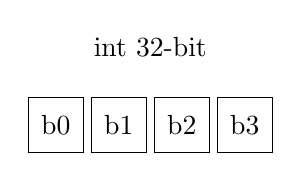
\begin{tikzpicture}[node distance=0.5cm]
    \tikzstyle{cell}=[draw, minimum width=0.7cm, minimum height=0.7cm]
    \node at (0,0) [cell] {b0};
    \node at (0.8,0) [cell] {b1};
    \node at (1.6,0) [cell] {b2};
    \node at (2.4,0) [cell] {b3};
    \node at (1.2,1) {int 32-bit};
  \end{tikzpicture}
  \caption{Contoh representasi integer 32-bit sebagai 4 byte}
\end{figure}

\section{Deklarasi \& Inisialisasi Variabel}
Deklarasi variabel berfungsi untuk menentukan nama, tipe data, dan scope dari variabel tersebut. Inisialisasi—yaitu pemberian nilai awal—sangat penting terutama di C untuk menghindari garbage value. C++ menawarkan uniform initialization dengan bracket yang lebih aman, sedangkan Pascal memiliki section \texttt{var} yang terpisah dan eksplisit \parencite{pascal-tutorial-wikibooks,gnu-c-manual,cpp-reference}.

\subsection{Contoh Deklarasi dan Inisialisasi}

Program-program berikut mendemonstrasikan bagaimana cara mendeklarasikan variabel dengan tipe data yang bervariasi dan memberikan nilai awal kepadanya:

\begin{lstlisting}[language=Pascal, caption={Deklarasi dan inisialisasi di Pascal}]
program Vars;
var
  count: integer = 0;
  ratio: double = 0.5;
  letter: char = 'A';
  flag: boolean = true;
begin
  Writeln(count, ' ', ratio:0:2, ' ', letter, ' ', flag);
end.
\end{lstlisting}

\begin{lstlisting}[language=C, caption={Deklarasi dan inisialisasi di C}]
#include <stdio.h>
int main(void) {
  int count = 0;
  double ratio = 0.5;
  char letter = 'A';
  _Bool flag = 1; // C99
  printf("%d %.2f %c %s\n", count, ratio, letter, flag?"true":"false");
  return 0;
}
\end{lstlisting}

\begin{lstlisting}[language=C++, caption={Deklarasi dan inisialisasi di C++}]
#include <iostream>
using namespace std;

int main() {
  int count{0};
  double ratio{0.5};
  char letter{'A'};
  bool flag{true};
  cout << count << ' ' << ratio << ' ' << letter << ' ' << boolalpha << flag << '\n';
}
\end{lstlisting}

Konsistensi dalam penamaan variabel akan meningkatkan readability kode secara signifikan. Jika scope sebuah variabel terlalu panjang, pertimbangkan untuk memecah fungsi menjadi unit-unit yang lebih kecil. Manfaatkan keyword \texttt{const} (atau padanannya) untuk mendefinisikan nilai-nilai yang sifatnya immutable.

Di C/C++, pemahaman tentang storage duration (automatic, static, dynamic) menjadi kunci dalam mengelola lifecycle variabel. Praktik terbaik adalah mendeklarasikan variabel sedekat mungkin dengan tempat penggunaannya untuk mengurangi cognitive load. Sementara di Pascal, pemisahan explicit melalui section \texttt{var} memberikan struktur yang lebih mudah untuk di-audit \parencite{free-pascal-docs,gnu-c-manual}.

\section{Input / Output Dasar}
Input dan output (I/O) adalah mekanisme yang memungkinkan program kita untuk berkomunikasi dengan user maupun file. Setiap bahasa memiliki pendekatan yang berbeda: Pascal menggunakan \texttt{Read/Readln} untuk input dan \texttt{Write/Writeln} untuk output; C mengandalkan \texttt{scanf} dan \texttt{printf}; sedangkan C++ menggunakan stream-based I/O dengan \texttt{std::cin} dan \texttt{std::cout}, dilengkapi dengan manipulator dari header \texttt{<iomanip>} \parencite{w3pascal-io,gnu-c-manual,cplusplus-io,cpp-iomanip}.

\subsection{Perbandingan Sintaks I/O Dasar}
\begin{table}[H]
  \centering
  \caption{Perbandingan ringkas perintah I/O}
  \label{tab:io-basic}
  \begin{tabular}{@{}lll@{}}
    \toprule
    Bahasa & Output & Input \\
    \midrule
    Pascal & \texttt{Writeln('...')} & \texttt{Readln(x)} \\
    C      & \texttt{printf("...")} & \texttt{scanf("\%d", \&x)} \\
    C++    & \texttt{std::cout << "..."} & \texttt{std::cin >> x} \\
    \bottomrule
  \end{tabular}
\end{table}

\subsection{Contoh Input/Output Dasar}
Berikut ini adalah contoh sederhana yang membaca dua angka integer dari user, menjumlahkannya, kemudian menampilkan hasilnya. Perhatikan bagaimana cara kerja I/O berbeda di masing-masing bahasa \parencite{w3pascal-io,gnu-c-manual,cpp-reference}.

Contoh pertama menunjukkan implementasi di Pascal—bagaimana kita membaca dua angka, melakukan penjumlahan, dan menampilkan output:

\begin{lstlisting}[language=Pascal, caption={Menjumlah dua bilangan pada Pascal}]
program SumTwo;
var
  a, b, total: integer;
begin
  Readln(a);
  Readln(b);
  total := a + b;
  Writeln('Jumlah = ', total);
end.
\end{lstlisting}

Implementasi yang ekuivalen di C memanfaatkan fungsi \texttt{scanf} untuk membaca input dan \texttt{printf} untuk menampilkan output:

\begin{lstlisting}[language=C, caption={Menjumlah dua bilangan pada C}]
#include <stdio.h>

int main(void) {
  int a, b;
  scanf("%d %d", &a, &b);
  printf("Jumlah = %d\n", a + b);
  return 0;
}
\end{lstlisting}

Di C++, pendekatan berbasis stream dengan operator \texttt{cin} dan \texttt{cout} menawarkan keamanan tipe yang lebih baik:

\begin{lstlisting}[language=C++, caption={Menjumlah dua bilangan pada C++}]
#include <iostream>
using namespace std;

int main() {
  int a, b;
  cin >> a >> b;
  cout << "Jumlah = " << (a + b) << '\n';
  return 0;
}
\end{lstlisting}

\begin{table}[H]
  \centering
  \small
  \caption{Instruksi Input/Output pada Pascal, C, dan C++}
  \begin{tabular}{@{}llll@{}}
    \toprule
    Operasi & Pascal & C & C++ \\
    \midrule
    Input standar & \texttt{Read()}, \texttt{Readln()} & \texttt{scanf()}, \texttt{fgets()} & \texttt{cin >>}, \texttt{getline()} \\
    Output standar & \texttt{Write()}, \texttt{Writeln()} & \texttt{printf()} & \texttt{cout <<} \\
    Output error & - & \texttt{fprintf(stderr)} & \texttt{cerr <<} \\
    Format output & \texttt{var:width:decimal} & \texttt{printf("\%format")} & manipulator \texttt{iomanip} \\
    Input string & \texttt{Readln(str)} & \texttt{fgets(...)} & \texttt{getline(...)} \\
    \bottomrule
  \end{tabular}
  \\\parencite{w3pascal-io,gnu-c-manual,cplusplus-io,cpp-iomanip}
\end{table}

Sebaiknya pisahkan error output (\texttt{stderr}) dari standard output untuk memfasilitasi automation dan debugging. Di C, manfaatkan \texttt{snprintf} sebagai alternatif yang lebih aman untuk menghindari buffer overflow. Sedangkan di C++, gunakan manipulator seperti \texttt{std::setw} dan \texttt{std::setprecision} untuk menghasilkan output yang terformat dengan rapi \parencite{gnu-c-manual,cpp-reference,cpp-iomanip}.

\subsection{Diagram Arus I/O}
\begin{figure}[H]
  \centering
  \begin{tikzpicture}[node distance=1.6cm, >=Stealth]
    \tikzstyle{box}=[rectangle, draw, rounded corners, align=center, minimum width=3.1cm, minimum height=1cm]
    \node[box] (kbd) {Keyboard/\newline Berkas Masuk};
    \node[box, right=of kbd] (prog) {Program};
    \node[box, right=of prog] (term) {Terminal/\newline Berkas Keluar};
    \draw[->] (kbd) -- node[above]{input} (prog);
    \draw[->] (prog) -- node[above]{output} (term);
  \end{tikzpicture}
  \caption{Arus I/O sederhana antara pengguna/berkas dan program}
  \label{fig:io-flow}
\end{figure}

\subsection{Contoh I/O Angka dan Pemformatan}

Program-program di bawah ini mengilustrasikan teknik memformat output angka—khususnya mengatur jumlah digit desimal—serta cara membaca input dari user:

\begin{lstlisting}[language=Pascal, caption={Baca integer dan format keluaran (Pascal)}]
program IOFmt;

var
  n: integer;
begin
  Write('Masukkan angka: ');
  Readln(n);
  Writeln('Kuadrat = ', n * n);
  Writeln('Pi ~ ', 3.14159:0:2);  // 2 digit desimal
end.
\end{lstlisting}

Dalam bahasa C, formatting output dilakukan dengan menentukan format specifier di dalam \texttt{printf}:

\begin{lstlisting}[language=C, caption={Baca integer dan format keluaran (C)}]
#include <stdio.h>
int main(void) {
  int n;
  printf("Masukkan angka: ");
  scanf("%d", &n);
  printf("Kuadrat = %d\n", n*n);
  printf("Pi ~ %.2f\n", 3.14159);
  return 0;
}
\end{lstlisting}

Untuk C++, kontrol terhadap format output dilakukan melalui manipulator yang tersedia di header \texttt{<iomanip>}:

\begin{lstlisting}[language=C++, caption={Baca integer dan format keluaran (C++)}]
#include <iostream>
#include <iomanip>
using namespace std;

int main() {
  int n;
  cout << "Masukkan angka: ";
  cin >> n;
  cout << "Kuadrat = " << n*n << "\n";
  cout << fixed << setprecision(2) << "Pi ~ " << 3.14159 << "\n";
  return 0;
}
\end{lstlisting}

\subsection{Contoh I/O String (Program Interaktif)}

Program-program interaktif berikut akan membaca nama dari user dan menampilkan pesan sambutan. Contoh ini menunjukkan bagaimana operasi I/O string bekerja di level dasar:

\begin{lstlisting}[language=Pascal, caption={Input nama pada Pascal}]
program Greet;

var
  name: string;
begin
  Write('Nama Anda? ');
  Readln(name);
  Writeln('Halo, ', name, '!');
end.
\end{lstlisting}

Pada bahasa C, input string ditangani dengan character array dan sebaiknya menggunakan fungsi \texttt{fgets} yang jauh lebih aman dibanding \texttt{gets}:

\begin{lstlisting}[language=C, caption={Input nama pada C}]
#include <stdio.h>
int main(void) {
  char name[64];
  printf("Nama Anda? ");
  fgets(name, sizeof name, stdin);
  printf("Halo, %s", name); // fgets menyertakan newline
  return 0;
}
\end{lstlisting}

C++ menyediakan \texttt{getline} yang bisa membaca string termasuk spasi di dalamnya, tidak seperti operator \texttt{>>} yang akan berhenti begitu menemui whitespace:

\begin{lstlisting}[language=C++, caption={Input nama pada C++}]
#include <iostream>
using namespace std;

int main() {
  char name[64];
  cout << "Nama Anda? ";
  cin.getline(name, sizeof(name));
  cout << "Halo, " << name << "!\n";
  return 0;
}
\end{lstlisting}

\subsection{Ringkasan Pemformatan}
\begin{table}[H]
  \centering
  \caption{Ringkasan pemformatan angka}
  \begin{tabular}{@{}lll@{}}
    \toprule
    Bahasa & Contoh & Keterangan \\
    \midrule
    Pascal & \texttt{real:0:2} & 2 digit desimal \\
    C & \texttt{"\textbackslash\%.2f"} & 2 digit desimal (\texttt{printf}) \\
    C++ & \texttt{std::fixed}, \texttt{std::setprecision(2)} & 2 digit desimal \\
    \bottomrule
  \end{tabular}
  \\\parencite{w3pascal-io,gnu-c-manual,cpp-iomanip}
\end{table}

\subsection{Cheat Sheet Format String (C)}
\begin{table}[H]
  \centering
  \caption{Specifier umum untuk \texttt{printf}/\texttt{scanf} (ringkas)}
  \small
  \begin{tabular}{@{}llll@{}}
    \toprule
    Nilai & \texttt{printf} & \texttt{scanf} & Catatan \\
    \midrule
    \texttt{int} & \texttt{\%d} & \texttt{\%d} & basis desimal \\
    \texttt{long} & \texttt{\%ld} & \texttt{\%ld} & \texttt{l} untuk long \\
    \texttt{long long} & \texttt{\%lld} & \texttt{\%lld} & \texttt{ll} untuk long long \\
    \texttt{unsigned} & \texttt{\%u} & \texttt{\%u} & tanpa tanda \\
    \texttt{double} & \texttt{\%f} & \texttt{\%lf} & beda antara printf dan scanf \\
    \texttt{char} & \texttt{\%c} & \texttt{\%c} & satu karakter \\
    string C & \texttt{\%s} & \texttt{\%s} & hati-hati overflow (batasi lebar) \\
    pointer & \texttt{\%p} & - & tampilkan alamat \\
    \bottomrule
  \end{tabular}
  \\\parencite{c-printf,c-scanf}
\end{table}

\paragraph{Tips.} Saat menggunakan \texttt{scanf}, selalu spesifikasikan maximum width seperti \texttt{"\%63s"} untuk buffer 64 byte guna mencegah overflow. Jangan lupa untuk memeriksa return value dari \texttt{scanf} untuk memverifikasi bahwa jumlah item yang berhasil di-parse sudah sesuai.

\subsection{Sinkronisasi I/O C++ dan Kinerja}
Secara default, stream I/O C++ (\texttt{iostream}) melakukan sinkronisasi dengan C's stdio library demi menjaga kompatibilitas. Jika Anda perlu performa yang lebih tinggi—terutama ketika handling input dalam jumlah besar—sinkronisasi ini bisa dimatikan dengan memanggil \texttt{ios::sync\_\allowbreak{}with\_\allowbreak{}stdio(false)} dan \texttt{cin.tie(nullptr)}. Namun perlu diingat: setelah dimatikan, jangan mencampur penggunaan stdio (seperti \texttt{printf/scanf}) dengan iostream dalam program yang sama. Untuk penjelasan teknis lebih detail, silakan lihat \parencite{cpp-sync-with-stdio}.

\section{Rangkuman Materi}
\begin{itemize}
  \item Kita telah membahas tipe data fundamental yang tersedia di Pascal, C, dan C++, serta perbedaan model data pada sistem 64-bit (LP64 versus LLP64).
  \item Tipe data fixed-width dari \texttt{<stdint.h>} atau \texttt{<cstdint>} diperkenalkan untuk portabilitas, bersama dengan cara query batasan nilai menggunakan \texttt{numeric\_limits}.
  \item Praktik deklarasi dan inisialisasi variabel telah dipelajari, termasuk perbedaan pendekatan I/O di ketiga bahasa pemrograman.
  \item Cheat sheet format specifier untuk C disertakan, lengkap dengan contoh parsing numerik yang reliable dan penjelasan tentang sinkronisasi I/O di C++.
  \item Visualisasi representasi memori untuk tipe 32-bit, pedoman type casting yang aman, serta troubleshooting tips untuk masalah-masalah umum.
\end{itemize}
\end{document}
